% 2013 年全国大纲卷文科第 9 题：y=sin(ωx+φ)（ω>0）的部分图象。
% 来源 PDF：普通高考/2013/2013大纲文(广西).pdf，第 1 页（印面 797）左栏。
% 图象最高点横坐标 x0，最低点横坐标 x0+π/4，两者相距半个周期。
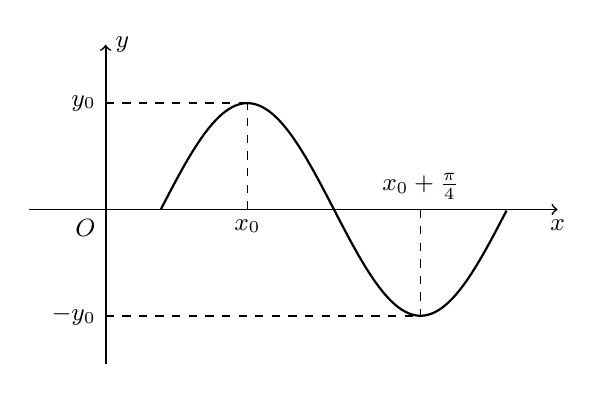
\begin{tikzpicture}[semithick, font=\small, x=2.8cm, y=1.35cm]
  \def\xz{0.6427}   % x0，最高点
  \def\xm{1.4284}   % x0+π/4，最低点
  \def\xs{0.25}     % 图象左端与 x 轴的交点
  % 坐标轴
  \draw[->] (-0.35,0) -- (2.05,0) node[below] {$x$};
  \draw[->] (0,-1.45) -- (0,1.55) node[right] {$y$};
  \node[below left] at (0,0) {$O$};
  % 最高点、最低点的虚线
  \draw[dashed] (0,1) -- (\xz,1);
  \draw[dashed] (\xz,0) -- (\xz,1);
  \draw[dashed] (0,-1) -- (\xm,-1);
  \draw[dashed] (\xm,0) -- (\xm,-1);
  % 正弦曲线
  \draw[thick, domain=\xs:1.8208, samples=240, smooth]
    plot (\x, {sin(4*(\x-\xs) r)});
  % 标注
  \node[left] at (0,1) {$y_0$};
  \node[left] at (0,-1) {$-y_0$};
  \node[below] at (\xz,0) {$x_0$};
  \node[above] at (\xm,0) {$x_0+\frac{\pi}{4}$};
\end{tikzpicture}
